\chapter{SP2-CU17 Agregar subrayado a propuesta de Unidad de Aprendizaje}
\begin{UseCase}{SP2-CU17}{ Agregar subrayado a propuesta de Unidad de Aprendizaje }{El usuario podrá agregar uno o más subrayados al texto en la sección de propuesta de Unidad de Aprendizaje que se está revisando.}
		\UCitem{Versión}{\color{Gray}1.0}
		\UCitem{Autor}{\color{Gray}Romero Ponce Mauricio Isaac}
		\UCitem{Supervisa}{\color{Gray}Parra Garcilazo Cinthya Dolores}
		\UCitem{Actor}{Analista}
		\UCitem{Propósito}{Asignar puntos importantes a revisar por medio de subrayados en la sección de lapropuesta de Unidad de Aprendizaje  que se está revisando.}
		\UCitem{Entradas}{Las dos entradas para agregar un subrayado en una sección de la propuesta de Unidad de Aprendizaje son:
          \begin{itemize}
          	\item Posición en la que se agregará el subrayado.
          	\item Texto que se subraya.
           % \item fecha en que se genera el nuevo comentario.
            %\item Identificador unico del analista.
          \end{itemize}
        }
		\UCitem{Origen}{Mouse}
		\UCitem{Salidas}{
        	\begin{itemize}
        		\hypertarget{MSG12}{\item MSG12. Error: Primero se debe seleccionar el punto en donde se agregará el subrayado.}
        	\end{itemize}
        }
		\UCitem{Destino}{Pantalla.}
		\UCitem{Precondiciones}{ Se llamó al caso de uso SP2-CU7 o SP2-CU8 o SP2-CU9 o SP2-CU10 o  SP2-CU11 o SP2-CU12}
		\UCitem{Postcondiciones}{
            \begin{itemize}
                \item Se agregará al sistema el subrayado.
                \item Se mostrará en el documento el subrayado en amarillo.
                \item Se habilita la llamada al caso de uso SP2-CU18.  
             \end{itemize}  
        }
		\UCitem{Errores}{}
		\UCitem{Estado}{Revisión.}
		\UCitem{Observaciones}{}
\end{UseCase}

%--------------------------- CU TRAYECTORIA PRINCIPAL -------------------------
\begin{UCtrayectoria}{Principal}

    \UCpaso[\UCactor] Selecciona con el mouse el texto donde pondrá un subrayado de texto.

    \UCpaso[\UCactor] Presiona el botón \IUbutton{Subrayar}. \hyperref[SP2-CU17-A]{Trayectoria A}. 
    
    \UCpaso Verifica que se haya subrayado una sección del texto. 
    
    \UCpaso A la sección del texto seleccionada se le agrega un color de resaltado de textos de color amarillo.

\end{UCtrayectoria}

%------------------------ CU TRAYECTORIA ALTERNARIVA A -------------------------
\label{SP2-CU17-A}
\begin{UCtrayectoriaA}{A}{El usuario no seleccionó alguna parte del texto.}

	\UCpaso El sistema detecta que no hay referencia en el texto para el subrayado.

  \UCpaso El sistema muestra el \MSGref{MSG12}{Error: Primero se debe seleccionar el punto en donde se agregará el subrayado}.

  \UCpaso[\UCactor] Cierra el mensaje presionando \IUbutton{Aceptar}.

  \UCpaso continúa en el paso 1 de la trayectoria principal del CU-V14.
\end{UCtrayectoriaA}

\chapter{Pantallas}
 \begin{figure}
  \centering
    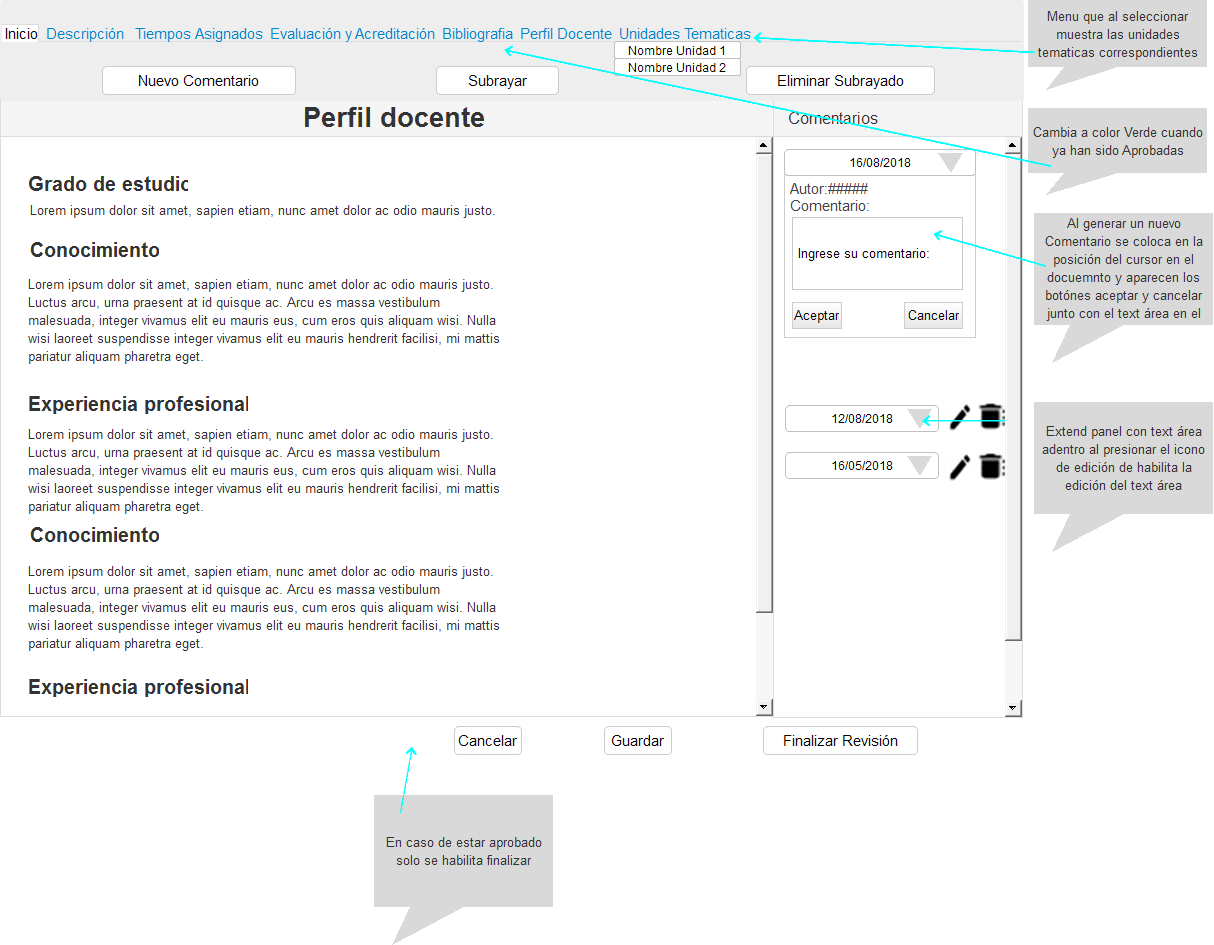
\includegraphics[width=0.7\textwidth]{DCU/SP2/Pantallas/Nuevo_comentario}
  \caption{SP2-IU-Nuevo comentario}
  \label{SP2-IU-Nuevo_comentario}
\end{figure}
